% Graphic for TeX using PGF
% Title: /home/thomas/work/src/github.com/bachopp/thesis/files/chapters/background/graphs/whole_system.dia
% Creator: Dia v0.97.3
% CreationDate: Tue May 10 13:45:51 2016
% For: thomas
% \usepackage{tikz}
% The following commands are not supported in PSTricks at present
% We define them conditionally, so when they are implemented,
% this pgf file will use them.
\ifx\du\undefined
  \newlength{\du}
\fi
\setlength{\du}{15\unitlength}
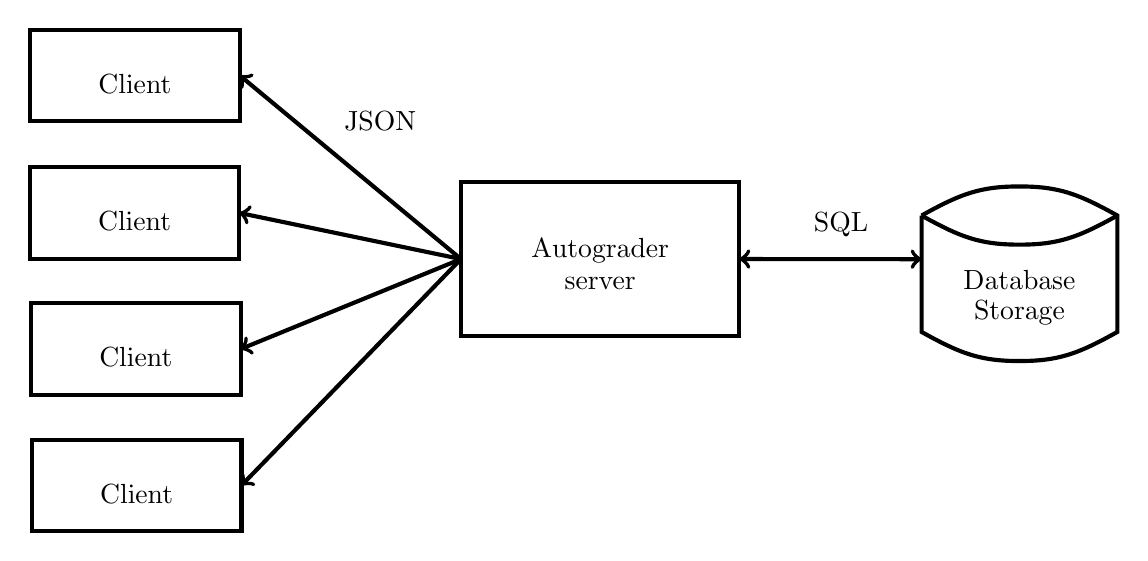
\begin{tikzpicture}
\pgftransformxscale{1.000000}
\pgftransformyscale{-1.000000}
\definecolor{dialinecolor}{rgb}{0.000000, 0.000000, 0.000000}
\pgfsetstrokecolor{dialinecolor}
\definecolor{dialinecolor}{rgb}{1.000000, 1.000000, 1.000000}
\pgfsetfillcolor{dialinecolor}
\definecolor{dialinecolor}{rgb}{1.000000, 1.000000, 1.000000}
\pgfsetfillcolor{dialinecolor}
\fill (15.721617\du,14.193104\du)--(15.721617\du,16.393104\du)--(20.771617\du,16.393104\du)--(20.771617\du,14.193104\du)--cycle;
\pgfsetlinewidth{0.100000\du}
\pgfsetdash{}{0pt}
\pgfsetdash{}{0pt}
\pgfsetmiterjoin
\definecolor{dialinecolor}{rgb}{0.000000, 0.000000, 0.000000}
\pgfsetstrokecolor{dialinecolor}
\draw (15.721617\du,14.193104\du)--(15.721617\du,16.393104\du)--(20.771617\du,16.393104\du)--(20.771617\du,14.193104\du)--cycle;
% setfont left to latex
\definecolor{dialinecolor}{rgb}{0.000000, 0.000000, 0.000000}
\pgfsetstrokecolor{dialinecolor}
\node at (18.246617\du,15.488104\du){Client};
\definecolor{dialinecolor}{rgb}{1.000000, 1.000000, 1.000000}
\pgfsetfillcolor{dialinecolor}
\fill (15.714354\du,17.505256\du)--(15.714354\du,19.705256\du)--(20.764354\du,19.705256\du)--(20.764354\du,17.505256\du)--cycle;
\pgfsetlinewidth{0.100000\du}
\pgfsetdash{}{0pt}
\pgfsetdash{}{0pt}
\pgfsetmiterjoin
\definecolor{dialinecolor}{rgb}{0.000000, 0.000000, 0.000000}
\pgfsetstrokecolor{dialinecolor}
\draw (15.714354\du,17.505256\du)--(15.714354\du,19.705256\du)--(20.764354\du,19.705256\du)--(20.764354\du,17.505256\du)--cycle;
% setfont left to latex
\definecolor{dialinecolor}{rgb}{0.000000, 0.000000, 0.000000}
\pgfsetstrokecolor{dialinecolor}
\node at (18.239354\du,18.800256\du){Client};
\definecolor{dialinecolor}{rgb}{1.000000, 1.000000, 1.000000}
\pgfsetfillcolor{dialinecolor}
\fill (15.743405\du,20.785619\du)--(15.743405\du,22.985619\du)--(20.793405\du,22.985619\du)--(20.793405\du,20.785619\du)--cycle;
\pgfsetlinewidth{0.100000\du}
\pgfsetdash{}{0pt}
\pgfsetdash{}{0pt}
\pgfsetmiterjoin
\definecolor{dialinecolor}{rgb}{0.000000, 0.000000, 0.000000}
\pgfsetstrokecolor{dialinecolor}
\draw (15.743405\du,20.785619\du)--(15.743405\du,22.985619\du)--(20.793405\du,22.985619\du)--(20.793405\du,20.785619\du)--cycle;
% setfont left to latex
\definecolor{dialinecolor}{rgb}{0.000000, 0.000000, 0.000000}
\pgfsetstrokecolor{dialinecolor}
\node at (18.268405\du,22.080619\du){Client};
\definecolor{dialinecolor}{rgb}{1.000000, 1.000000, 1.000000}
\pgfsetfillcolor{dialinecolor}
\fill (15.763405\du,24.070507\du)--(15.763405\du,26.270507\du)--(20.813405\du,26.270507\du)--(20.813405\du,24.070507\du)--cycle;
\pgfsetlinewidth{0.100000\du}
\pgfsetdash{}{0pt}
\pgfsetdash{}{0pt}
\pgfsetmiterjoin
\definecolor{dialinecolor}{rgb}{0.000000, 0.000000, 0.000000}
\pgfsetstrokecolor{dialinecolor}
\draw (15.763405\du,24.070507\du)--(15.763405\du,26.270507\du)--(20.813405\du,26.270507\du)--(20.813405\du,24.070507\du)--cycle;
% setfont left to latex
\definecolor{dialinecolor}{rgb}{0.000000, 0.000000, 0.000000}
\pgfsetstrokecolor{dialinecolor}
\node at (18.288405\du,25.365507\du){Client};
\definecolor{dialinecolor}{rgb}{1.000000, 1.000000, 1.000000}
\pgfsetfillcolor{dialinecolor}
\fill (26.102043\du,17.869764\du)--(26.102043\du,21.564019\du)--(32.808654\du,21.564019\du)--(32.808654\du,17.869764\du)--cycle;
\pgfsetlinewidth{0.100000\du}
\pgfsetdash{}{0pt}
\pgfsetdash{}{0pt}
\pgfsetmiterjoin
\definecolor{dialinecolor}{rgb}{0.000000, 0.000000, 0.000000}
\pgfsetstrokecolor{dialinecolor}
\draw (26.102043\du,17.869764\du)--(26.102043\du,21.564019\du)--(32.808654\du,21.564019\du)--(32.808654\du,17.869764\du)--cycle;
% setfont left to latex
\definecolor{dialinecolor}{rgb}{0.000000, 0.000000, 0.000000}
\pgfsetstrokecolor{dialinecolor}
\node at (29.455348\du,19.511892\du){Autograder};
% setfont left to latex
\definecolor{dialinecolor}{rgb}{0.000000, 0.000000, 0.000000}
\pgfsetstrokecolor{dialinecolor}
\node at (29.455348\du,20.311892\du){server};
\pgfsetlinewidth{0.100000\du}
\pgfsetdash{}{0pt}
\pgfsetdash{}{0pt}
\pgfsetbuttcap
\pgfsetmiterjoin
\pgfsetlinewidth{0.100000\du}
\pgfsetbuttcap
\pgfsetmiterjoin
\pgfsetdash{}{0pt}
\definecolor{dialinecolor}{rgb}{1.000000, 1.000000, 1.000000}
\pgfsetfillcolor{dialinecolor}
\pgfpathmoveto{\pgfpoint{37.198062\du}{18.668558\du}}
\pgfpathcurveto{\pgfpoint{38.141350\du}{18.142810\du}}{\pgfpoint{38.612993\du}{17.967561\du}}{\pgfpoint{39.556281\du}{17.967561\du}}
\pgfpathcurveto{\pgfpoint{40.499569\du}{17.967561\du}}{\pgfpoint{40.971212\du}{18.142810\du}}{\pgfpoint{41.914500\du}{18.668558\du}}
\pgfpathlineto{\pgfpoint{41.914500\du}{21.472548\du}}
\pgfpathcurveto{\pgfpoint{40.971212\du}{21.998296\du}}{\pgfpoint{40.499569\du}{22.173545\du}}{\pgfpoint{39.556281\du}{22.173545\du}}
\pgfpathcurveto{\pgfpoint{38.612993\du}{22.173545\du}}{\pgfpoint{38.141350\du}{21.998296\du}}{\pgfpoint{37.198062\du}{21.472548\du}}
\pgfpathlineto{\pgfpoint{37.198062\du}{18.668558\du}}
\pgfusepath{fill}
\definecolor{dialinecolor}{rgb}{0.000000, 0.000000, 0.000000}
\pgfsetstrokecolor{dialinecolor}
\pgfpathmoveto{\pgfpoint{37.198062\du}{18.668558\du}}
\pgfpathcurveto{\pgfpoint{38.141350\du}{18.142810\du}}{\pgfpoint{38.612993\du}{17.967561\du}}{\pgfpoint{39.556281\du}{17.967561\du}}
\pgfpathcurveto{\pgfpoint{40.499569\du}{17.967561\du}}{\pgfpoint{40.971212\du}{18.142810\du}}{\pgfpoint{41.914500\du}{18.668558\du}}
\pgfpathlineto{\pgfpoint{41.914500\du}{21.472548\du}}
\pgfpathcurveto{\pgfpoint{40.971212\du}{21.998296\du}}{\pgfpoint{40.499569\du}{22.173545\du}}{\pgfpoint{39.556281\du}{22.173545\du}}
\pgfpathcurveto{\pgfpoint{38.612993\du}{22.173545\du}}{\pgfpoint{38.141350\du}{21.998296\du}}{\pgfpoint{37.198062\du}{21.472548\du}}
\pgfpathlineto{\pgfpoint{37.198062\du}{18.668558\du}}
\pgfusepath{stroke}
\pgfsetbuttcap
\pgfsetmiterjoin
\pgfsetdash{}{0pt}
\definecolor{dialinecolor}{rgb}{0.000000, 0.000000, 0.000000}
\pgfsetstrokecolor{dialinecolor}
\pgfpathmoveto{\pgfpoint{37.198062\du}{18.668558\du}}
\pgfpathcurveto{\pgfpoint{38.141350\du}{19.194306\du}}{\pgfpoint{38.612993\du}{19.369556\du}}{\pgfpoint{39.556281\du}{19.369556\du}}
\pgfpathcurveto{\pgfpoint{40.499569\du}{19.369556\du}}{\pgfpoint{40.971212\du}{19.194306\du}}{\pgfpoint{41.914500\du}{18.668558\du}}
\pgfusepath{stroke}
% setfont left to latex
\definecolor{dialinecolor}{rgb}{0.000000, 0.000000, 0.000000}
\pgfsetstrokecolor{dialinecolor}
\node at (39.556281\du,20.221052\du){Database};
% setfont left to latex
\definecolor{dialinecolor}{rgb}{0.000000, 0.000000, 0.000000}
\pgfsetstrokecolor{dialinecolor}
\node at (39.556281\du,21.021052\du){Storage};
\pgfsetlinewidth{0.100000\du}
\pgfsetdash{}{0pt}
\pgfsetdash{}{0pt}
\pgfsetmiterjoin
\pgfsetbuttcap
{
\definecolor{dialinecolor}{rgb}{0.000000, 0.000000, 0.000000}
\pgfsetfillcolor{dialinecolor}
% was here!!!
\pgfsetarrowsstart{to}
{\pgfsetcornersarced{\pgfpoint{0.000000\du}{0.000000\du}}\definecolor{dialinecolor}{rgb}{0.000000, 0.000000, 0.000000}
\pgfsetstrokecolor{dialinecolor}
\draw (20.771617\du,15.293104\du)--(26.102043\du,19.716892\du);
}}
\pgfsetlinewidth{0.100000\du}
\pgfsetdash{}{0pt}
\pgfsetdash{}{0pt}
\pgfsetmiterjoin
\pgfsetbuttcap
{
\definecolor{dialinecolor}{rgb}{0.000000, 0.000000, 0.000000}
\pgfsetfillcolor{dialinecolor}
% was here!!!
\pgfsetarrowsstart{to}
{\pgfsetcornersarced{\pgfpoint{0.000000\du}{0.000000\du}}\definecolor{dialinecolor}{rgb}{0.000000, 0.000000, 0.000000}
\pgfsetstrokecolor{dialinecolor}
\draw (20.764354\du,18.605256\du)--(26.102043\du,19.716892\du);
}}
\pgfsetlinewidth{0.100000\du}
\pgfsetdash{}{0pt}
\pgfsetdash{}{0pt}
\pgfsetmiterjoin
\pgfsetbuttcap
{
\definecolor{dialinecolor}{rgb}{0.000000, 0.000000, 0.000000}
\pgfsetfillcolor{dialinecolor}
% was here!!!
\pgfsetarrowsstart{to}
{\pgfsetcornersarced{\pgfpoint{0.000000\du}{0.000000\du}}\definecolor{dialinecolor}{rgb}{0.000000, 0.000000, 0.000000}
\pgfsetstrokecolor{dialinecolor}
\draw (20.793405\du,21.885619\du)--(26.102043\du,19.716892\du);
}}
\pgfsetlinewidth{0.100000\du}
\pgfsetdash{}{0pt}
\pgfsetdash{}{0pt}
\pgfsetmiterjoin
\pgfsetbuttcap
{
\definecolor{dialinecolor}{rgb}{0.000000, 0.000000, 0.000000}
\pgfsetfillcolor{dialinecolor}
% was here!!!
\pgfsetarrowsstart{to}
{\pgfsetcornersarced{\pgfpoint{0.000000\du}{0.000000\du}}\definecolor{dialinecolor}{rgb}{0.000000, 0.000000, 0.000000}
\pgfsetstrokecolor{dialinecolor}
\draw (20.813405\du,25.170507\du)--(26.102043\du,19.716892\du);
}}
% setfont left to latex
\definecolor{dialinecolor}{rgb}{0.000000, 0.000000, 0.000000}
\pgfsetstrokecolor{dialinecolor}
\node[anchor=west] at (23.018654\du,16.388469\du){JSON};
\pgfsetlinewidth{0.100000\du}
\pgfsetdash{}{0pt}
\pgfsetdash{}{0pt}
\pgfsetbuttcap
{
\definecolor{dialinecolor}{rgb}{0.000000, 0.000000, 0.000000}
\pgfsetfillcolor{dialinecolor}
% was here!!!
\pgfsetarrowsstart{to}
\pgfsetarrowsend{to}
\definecolor{dialinecolor}{rgb}{0.000000, 0.000000, 0.000000}
\pgfsetstrokecolor{dialinecolor}
\draw (32.808654\du,19.716892\du)--(37.198062\du,19.720054\du);
}
% setfont left to latex
\definecolor{dialinecolor}{rgb}{0.000000, 0.000000, 0.000000}
\pgfsetstrokecolor{dialinecolor}
\node[anchor=west] at (34.332603\du,18.879300\du){SQL};
\end{tikzpicture}
